% Euclidean Handout Number fifteen
\documentclass{tufte-handout}

%\geometry{showframe}% for debugging purposes -- displays the margins

%%%% Packages to make things pretty
\usepackage{amsmath,amsthm}
\usepackage{booktabs}
\usepackage{graphicx}
\setkeys{Gin}{width=\linewidth,totalheight=\textheight,keepaspectratio}
\graphicspath{{graphics/}}
\usepackage{units}
\usepackage{fancyvrb}
\fvset{fontsize=\normalsize}
\usepackage{multicol}
\usepackage{pdfpages}

%%%% Theorem Evironments
\theoremstyle{definition}
\swapnumbers
\newtheorem{problem}{Problem}[section]
\newtheorem{conjecture}[problem]{Conjecture}
\newtheorem*{definition}{Definition}
\newtheorem*{theorem}{Theorem}
\newtheorem{question}[problem]{Question}
\newtheorem{challenge}[problem]{Challenge}
\newtheorem*{postulate}{Postulate}

%%%%%

\title{Euclidean Geometry:\\An Introduction to Mathematical Work}
\author[]{Math 3600}
\date{Fall 2015}

\begin{document}

\maketitle

\begin{marginfigure}
    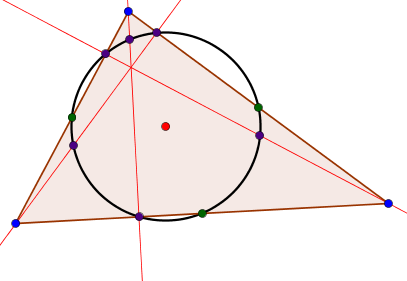
\includegraphics{NPC}
\end{marginfigure}

\setcounter{section}{15}
\section{Regular Figures, especially the Pentagon}

Read Book IV of the \emph{Elements}. Pay particular attention to propositions 10-12.

\begin{problem}\label{prob:GSP-reg-pentagon}
Prepare a presentation of Euclid's construction of a regular pentagon.
\end{problem}

\begin{problem}\label{prob:circle-inscribe-triangle} Given a circle, but not its center, construct an inscribed equilateral triangle in as few steps as possible. (par 7)
\end{problem}

\begin{problem}\label{prob:square}
Construct a square in as few steps as possible. (par 9)
\end{problem}

\begin{problem}\label{prob:side-reg-pent}
Given a line segment $AB$, construct a regular pentagon having $AB$ as a side. (par 11)
\end{problem}

\begin{problem}\label{prob:circle-three-tangent-circles}
Given a circle $\Gamma$ and its center $O$, construct inside $\Gamma$ three equal circles, each one tangent to $\Gamma$ and to the other two. (par 13)
\end{problem}

\begin{problem}\label{prob:inscribed-circle-content}
Let $ABC$ be an equilateral triangle inscribed in a circle. Let $D$ and $E$ be the midpoints of two sides, and extend segment $DE$ to meet the circle at $F$ so that $E$ lies between $D$ and $F$. Show that the rectangle on $EF$ and $DF$ has the same content as the square on $DE$.
\end{problem}

%\begin{problem}\label{prob:paper-pentagon}
%Take a long, thing piece of paper, tie a simple overhand knot in the paper and fold the knot flat. The flat knot makes a regular pentagon. Explain!
%\end{problem}

\begin{challenge}\label{chal:hexagon}
Construct a regular hexagon in as few steps as possible. What should the par value be?
\end{challenge}

\vfill
\end{document}
